\documentclass[12pt]{article}
\usepackage{listings}
\usepackage[utf8]{inputenc}
\usepackage{geometry}
\usepackage{fancyhdr}
\usepackage{xcolor}
\usepackage{hyperref}
\usepackage{subcaption}
\usepackage{graphicx}
\usepackage[absolute,overlay]{textpos}
\usepackage{titling}

\geometry{
    a4paper,
    total={170mm,257mm},
    left=20mm,
    top=10mm,
}

\hypersetup{
    colorlinks=true,
    linkcolor=blue,
    filecolor=magenta,      
    urlcolor=cyan,
}


\definecolor{codegreen}{rgb}{0,0.6,0}
\definecolor{codegray}{rgb}{0.5,0.5,0.5}
\definecolor{codepurple}{rgb}{0.58,0,0.82}
\definecolor{backcolour}{rgb}{0.95,0.95,0.92}

\lstdefinestyle{mystyle}{
    backgroundcolor=\color{backcolour},   
    commentstyle=\color{codegreen},
    keywordstyle=\color{magenta},
    numberstyle=\tiny\color{codegray},
    stringstyle=\color{codepurple},
    basicstyle=\ttfamily\footnotesize,
    breakatwhitespace=false,         
    breaklines=true,                 
    captionpos=b,                    
    keepspaces=true,                 
    numbers=left,                    
    numbersep=5pt,                  
    showspaces=false,                
    showstringspaces=false,
    showtabs=false,                  
    tabsize=2
}

\lstset{style=mystyle}

\begin{document}
\setlength{\droptitle}{-4em}

\title{Comparing Regression Models for Electron Mass Prediction\vspace{-2em}}
\date{\today\vspace{-1em}}
\maketitle

\section{Introduction}
In this project, we are looking into the topic of particle physics, specifically focusing on electron events conducted by CERN in 2010. These events involve collisions of particles, resulting in a large amount of data of such collisions involving dielectrons. Our primary objective is to predict the mass of electrons based on the available dataset for each event. To achieve this, we empoly Machine Learning by utilizing the labeled data provided in the dataset to train a predictive model. This report is structured as follows: first, we introduce the problem formulation and feature selection, outlining the dataset and data preprocessing steps. Next, we move into our models and feature selection process, discussing the relevant attributes and the reasoning behind choosing our prospective regression models for our specific case. Our goal is to take advantage of the benefits of machine learning to gain insights into the world of particle physics and make accurate predictions about electron masses in these collision events.


\section{Problem Formulation and Feature selection}


In This project we are dealing with a series of \textit{events} of electrons accomplished by CERN in 2010. 
Events are thereby defined as a collision of particles.
During this series data of 100.000 collisions between electrons were collected. The electrons in this events had an invariant mass in a range of 2 and 110 GeV.\cite{mccauley_dielectron_2016}\\
Following, we want to predict the mass of the electrons based on the given data of each event. We opt for supervised learning in our project because we aim to predict the mass of electrons based on the provided dataset of events, where the actual mass values are available (labeled data). Supervised learning allows us to train a predictive model using the labeled data, enabling it to make mass predictions for new unseen events.

\subsection{Data Description and Data Prepossessing}

We are using the dataset of this series provided by the "Open Data Portal" from CERN. The dataset includes 19 features, as shown in the tables below. %The features are: run number (Int); event number (Int); mass (float) and each for both electrons: energy of the electrons (float); momentum of the electron given by a feature for x,y and z values (float); transverse momentum (float); pseudo rapidity (float); phi angle (float); charge ($\{-1,1\}$). All Float values are (GeV) but the phi which are (rad). More details in Table below.\\
%\newpage
\begin{figure}[h]
\centering
\begin{subfigure}{0.5\textwidth}
  \centering
  %\caption{Description of Dataset(Electron 1)}
  \begin{tabular}{|c|c|c|}
    \hline
    \textbf{Feature} & \textbf{Description} & \textbf{Type} \\
    \hline
    Run & run number & Int\\
    Event & event number & Int\\
    E1 & total energy  & Float\\
    E2 & total energy  & Float\\
    px1 & x component  & Float\\
    py1 & y component  & Float\\
    pz1 & z component  & Float\\
    px2 & x component & Float\\
    py2 & y component & Float\\
    pz2 & z component & Float\\
    
    \hline
  \end{tabular}
\end{subfigure}%
\begin{subfigure}{0.5\textwidth}
  \centering
  %\caption{Description of Dataset(Electron 2)}
  \begin{tabular}{|c|c|c|}
    \hline
    \textbf{Feature} & \textbf{Description} & \textbf{Type} \\
    \hline
    pt1 & transverse momentum  & Float\\
    pt2 & transverse momentum  & Float\\
    eta1 & pseudorapidity  & Float\\
    eta2 & pseudorapidity  & Float\\
    phi1 & phi angle & Float\\
    phi2 & phi angle  & Float\\
    Q1 & charge & \{-1, 1\}\\ 
    Q2 & charge  & \{-1, 1\}\\
    M & Invariant Mass & Float\\
    \hline
  \end{tabular}
\end{subfigure}
\end{figure}
\newpage
The dataset consists of 100.000 entries thus making it a large dataset. In order to correctly apply machine learning methods to our dataset we have to apply some prepossessing techniques. In this way we are ensuring data quality, noise reduction and making it more suitable for model training.\cite{scikit-learn-Preprocessing}\\

We begin with examining the dataset and looking for missing or duplicate values. By dropping the duplicate values we ensure data integrity and prevent redundancy, while removing null values helps maintain data consistency and prevents potential issues in model training. While the number of data dropped in total is relatively small to the total size of features, this common practise technique is applied in order to achieve the best possible results.


\section{Models and Feature Selection}

\subsection{Feature Selection and Analysis}
For the feature selection stage we went through a process of determining the features that are going to end up being the important ones for our model. In order to do that we:

\begin{enumerate}
    \item Generated a heatmap that's showing the correlation of each feature with the target.
    \item Generated useful scatter plots between Mass and each other feature.
\end{enumerate}

After examining the above graphs, we noticed et1, et2 as well as Q1 and Q2 and both phi angles do not offer much of help on determining the Mass as there absolutely no geometrical correlation  between the 2 factors. By further examining the heatmap we noticed a high correlation between E1,E2 as well as pt1 and pt2. When we are dealing with supervised model, highly correlated values will not improve the results. For linear models large correlation can lead to unstable results and can cause large variations. Moreover, although random forests model works very well on distinguishing those features, keeping them can mask this ability.\\
For the above mentioned reasons, for our case study and experiment we ended up using the components of the electron 1 and 2, that is \textit{px}, \textit{py} and \textit{pz}. Finally, we used boxplot graphs to analyze our selected features and identified the presence of outliers. However, since the number of instances with outliers was small, we decided to retain them in our analysis.


\subsection{Models}

The are many machine learning models that are used for accurate target predictions in supervised learning but not all of them work best for all cases. For this reason, we had to select our model based on our case study and our dataset. The two models that we are going to investigate in our report are \textbf{Random Forest Regression}, \textbf{Decision tree regression} and \textbf{MLP Regression}. In more detail we will look through the thought process lead to the choosing model for our case:


\underline{\vspace{0.5em}}

\underline{\textbf{Random Forest Regression (RFG)}}\\
By utilizing this model, we can take advantage of its robustness to outliers, which is highly beneficial since that during the prepossessing phase, we did not perform any outlier removal.
Moreover, it uses multiple decision trees, each trained for a subset of the data, thus being more likely to find a more optimal solution than a local optimal. It's also worth noting that by drooping features on the feature selection part we are more likely to overfit since our model is getting trained on a fewer specimens which are less diverse, so Random Forests offers an advantage to that since it is robust to overfit. Lastly, having already notices the non-linear nature of our dataset, we are considering this model for its good performance with such datasets.\cite{scikit-learn-RandomForestRegressor}\\


\underline{\textbf{Decision Tree Regression (DTR)}}\\
Decision trees are renowned for their robust performance with large datasets, making them an ideal choice for our needs given the scale of our dataset. Furthermore, their versatility extends beyond standard predictions, making them readily adaptable to our specific case. Another notable advantage of this method lies in its intuitive and easily comprehensible nature, making it straightforward to apply in addressing our problem.\cite{scikit-learn-DecisionTreeRegressor}\\


\underline{\textbf{Multi-layer Perceptron Regressor (MLP)}}\\
The Multi-layer perceptron regression model is using an artificial neural network of multiple layers of perceptrons. This regression model is good at capturing complex non-linear relationships within our dataset. In order to prevent overfitting we carefully fine-tune its hyperparameters in the following sections. Its adaptability to diverse attributes is particularly advantageous for our dataset, making the MLP Regressor a robust choice.\cite{scikit-learn-MLPRegressor}




\subsection{Loss Function}


\underline{\textbf{Mean Squared Error}}

One compelling reason to use this loss function is its ability to decrease the impact of outliers. Outliers can lead to significantly larger error values because of the squaring operation in the Mean Squared Error (MSE) formula:

\vspace{0.2em}

\begin{center}
$MSE = \frac{1}{n} \sum_{i=1}^{n}(y_i - \hat{y}_i)^2$
\end{center}
\vspace{0.2em}


As a result, when encountering outliers, the MSE increase their influence on the overall error, making it easier to identify and disregard them in the modeling process. Moreover, the mean squared error function is chosen as it allowed us to use the already made library from \textit{sklearn}, as it is the default function of our models and the most widely used one.\cite{chai_root_2014}


\section{Model Validation}
To validate the result of our model we splitted our data with \textit{train\_test\_split} from \textit{sklearn} into training, validation and test-set with a ratio of 0.8/0.1/0.1. We were able to afford such a big training-set because of our large dataset, by which we can ensure enough data for our validation and test-set.\\
After we trained our model with our training-set we tuned the hyperparameters of our models with the validation-set to improve the performance of the chosen models. At the end we compare the models by predicting labels over the test-set and comparing these with the labels of our test-set by the MSE.


\section{Results}
After prepossessing the data we initially trained our models with the training-set and the default parameters provided by \textit{sklearn}. Moving on, we are predicting with each model on the training-set and validation-set and computing the training and test-error. Obtaining these, allows us to compare the two models for the first time. It's clearly visible, DTR model is overfitting a lot compared to our RFG model. More specifically training-error of the DTR model equals to zero and the validation-error is $\sim47.854$. On the other hand the training-error of the RFG model is $\sim2.535$ and validation-error is $\sim18.045$, indicating less overfitting. 
Introducing MLP model to the comparison, it's training-error during the initial prediction is $\sim10.375$ and the validation-error is $\sim12.716$.
Based on these results, we are going to focus on RFG and MLP as they deliver better validation-error performance and less overfitting.\\
For both models, we used the \textit{GridSearchCV} from \textit{sklearn} to tune our hyper-parameter on the validation-set.\cite{scikit-learn-GridSearchCV}. This enables us to find better fitting parameters for our dataset and improve the performance. As a result we improve the validation-error of RFG model to $\sim5.116$ and $\sim2.288$ respectively.\\

Continuing our comparison, we are also going through the test-error results. As aforementioned, we randomly split the training-set from the original dataset with a ratio of $10\%$. It's important that we never used it to train our models to provide a good comparison.\\

The final results are very impressive supported by the fact the MLP model is showing a very precise prediction on the test-set. The RFG model obtained a final test-error of $\sim4.498$ and the MLP model a test-error of $\sim2.056$.\\

\section{Conclusion }
All in all, we can see that the MLP model reaches the best performance in the end. The test-error doesn't differ from the training-error on such a large scale the RFG model does. This indicates that our RFG model still suffers from overfitting. On the other hand, RFG model is much faster. During the final run, it needed approximately $1.5$ minutes to train and predict, whereas MLP model needed over $15$ minutes.\\
In the following graph, we compare the two models by their residual plot. It's getting clear, that the outliers of MLP model are not as distant to real labels as is the case for the RFG model.
\begin{center}
  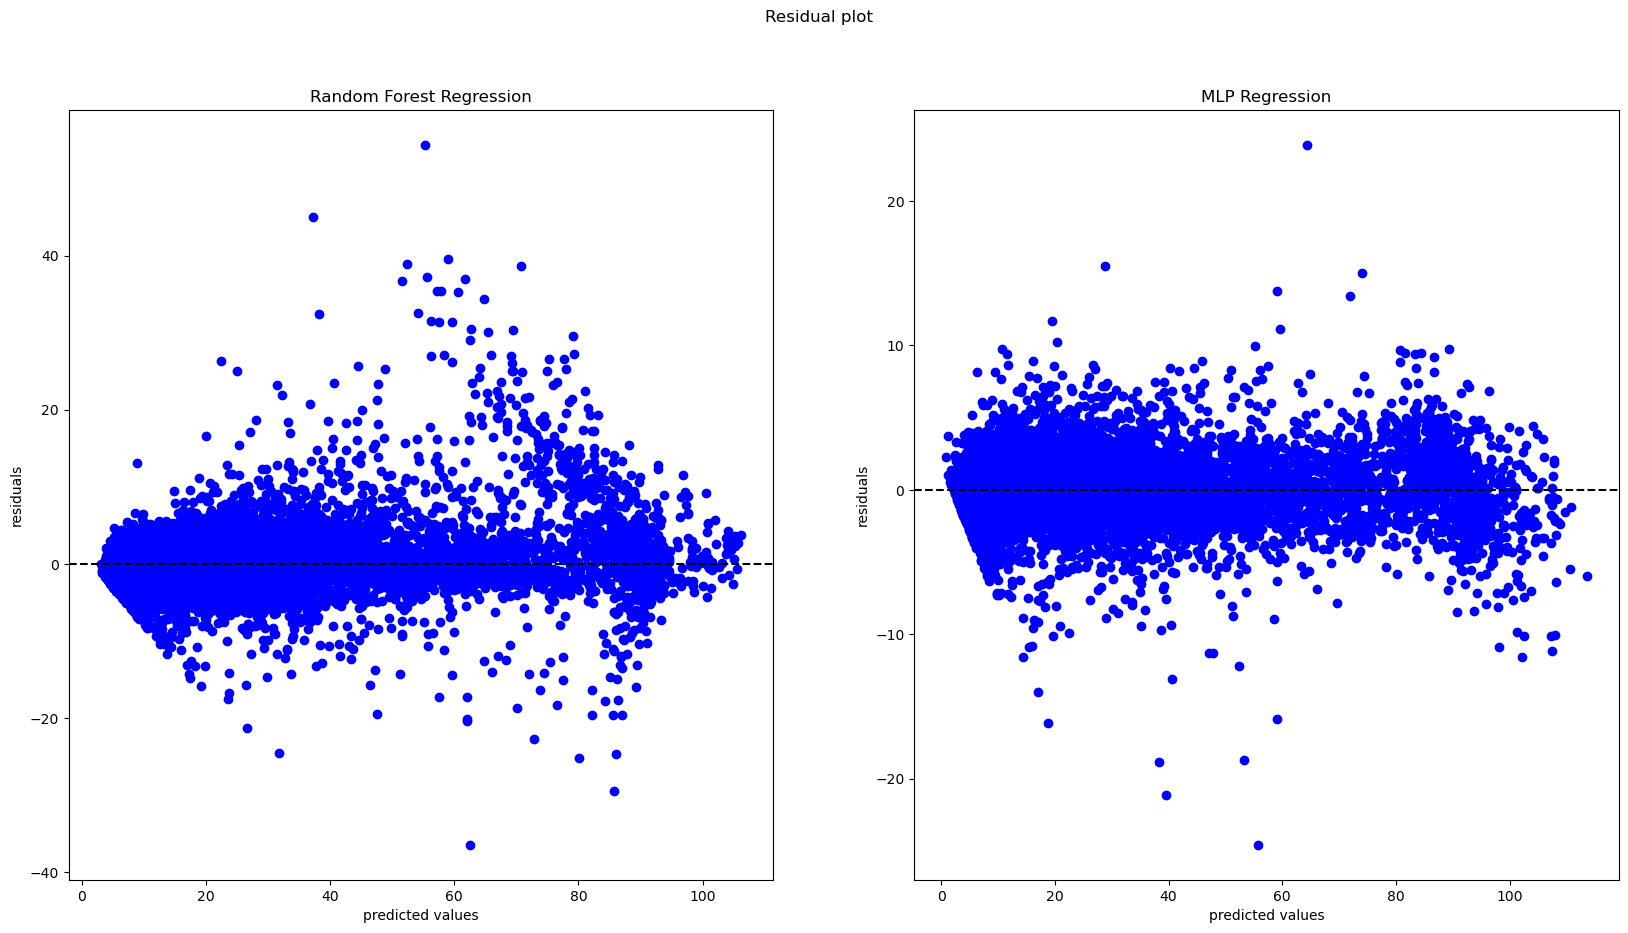
\includegraphics[height=6cm]{Residual_Plot.png}
\end{center}
Equally noteworthy, is the performance increase of the MLP model by the higher number of maximum iterations. Should one train it for longer the result would still improve, contrary to the fact that RFG model wouldn't improve on such a scale by increasing the number of estimators.\\

To draw the discussion to a close, for the current case study the MLP model showed the best performance, indicating further improvements by training it for a bigger span of time and therefore stands out as the best fitting model to predict the invariant mass in our dataset.

\newpage
\bibliography{bib}
\nocite{cern-electron-collision-data}
\bibliographystyle{ieeetr}
\end{document}


